\chapter{Speech Processing}\label{ch:speech_processing}
Speech is an effortless and highly efficient form of communication.
Continuous speech recognition software is readily available from stores and it allows the user to interact with its surrounding without the need of written commands
\cite[p.~396]{callan2003artificial}. Amazon`s Alexa 
\cite{Alexa} and Microsoft`s Cortana 
\cite{Cortana} are perfect examples of home companions that are able to perform basic tasks received via voice commands.\\\\
As speech recognition increases in accuracy to the high nineties, reaching a performance of 99\%, \todo{find reference for 99} means that this technology will make the leap from being annoying to use, to becoming the main way we interact with computers. 
This idea is further backed up by the fact that people tend to speak much faster than they are able to type \cite{Speed}.
In some cases, speech can be three times faster in conveying information than typing, and for professional debaters,
speaking can be even six times faster.d
\todo{We looked over until here...}

\section{Classical overview}
Words are carried as sound waves, which are analogue signals.
In order for the speech to be processed,
it needs to be run through a signal processor that selects the frequencies and amplitude of the signal.
Further on, the signal is mapped to individual sound units called phones.
These phones need to be identified and grouped in such a way to ensure that each word has a different phonetic structure,
otherwise, words would be impossible to distinguish from one another.
\begin{table}[H]
\centering
	\caption{Phones.}
	\label{my-label}
	\begin{tabular}{l l}
		{[}ay{]} & \underline{ir}is \\
		{[}b{]}  & \underline{b}in  \\
		{[}er{]} & \underline{bir}d \\
		{[}l{]}  & \underline{l}ip  \\
		{[}p{]}  & \underline{p}in  \\
		{[}th{]} & \underline{thi}n
	\end{tabular}
\end{table}
Phones can have different sounds depending on the context. 
For example, the phone \textbf{th} in the word \textit{three} has a different sound to \textbf{th} in \textit{then}. 
To overcome these different variations of the same phones, 
it is better to abstract the phones into a generalized grouping called a \textbf{phoneme}.
Phonemes are written in-between forward slashes
(\textit{/th/}) and they will have a specific pronunciation for each sound, depending on the context.
These phonemes are used as a transitional layer when trying to convert speech to text and vice versa,
when speech needs to be synthesized.

\section{Signal processing}
Sound waves that carry human speech are variations in air pressure.
The key components of a sound wave are its \textbf{amplitude},
which measure the intensity of the sound and the \textbf{frequency}, which describes the rate at which the amplitude varies over time.
When speaking in a microphone,
the change in air pressure causes the diaphragm to oscillate.
The size of the oscillations is directly proportional to the amplitude of the signal,
while the rate at which the diaphragm oscillates gives represents the rate at which the air pressure changes.
At specific time intervals,
the signal can be sampled and the data can be used in a wide array of digital signal processing tools.
For example, the digital signal can be plotted as an x-y plot,
where the y-axis defines the amplitude and the x-axis shows the time.
The frequency can be easily be determined from the plot as we find the number of cycles that the signal does per second.\\\\
Although a visual difference can be seen when plotting vowels and consonants,
a visual inspection of the waveform will not reveal any critical information, making it impossible to see all the phonemes.\\\\
To feed this information to the neural network, some preprocessing and signal manipulation is required so the input can be understood and passed through the neurons.
These steps are expanded upon in the following subsections.

\subsubsection{ Preprocessing}
No matter how powerful and how advanced a computer is,
it still works in discrete time.
In order to represent an analogue signal on the computer, it has to be sampled according to the Nyquist–Shannon sampling theorem.
This theorem states that the sampling frequency has to be at least double the frequency of the original signal in order to replicate the original signal without aliasing.
For a better understanding of the process, a visual representation of the word "Hello" as it is formed for the input of the neural network is shown in the upper part of Figure\ref{fig:cyka}.

\subsubsection{ Fourier transform}
To analyse a discrete signal we use the Fourier transform. 
This allows us to convert the signal in the frequency domain and deconstruct it in a series of simple sine waves. 
These sine waves have specific amplitudes and frequencies and while plotting the FFT of the signal, 
the dominant waves can be identified by the intensity of the amplitude.\\\\
In the lower part of Figure \ref{fig:cyka}, a visual representation of the FFT is shown. 
It can be seen that there are a lot of frequencies that make up the word "Hello". 
The dominant ones are in the range of 500Hz. 
Considering that this recording has a minimum amount of noise,
we have to consider the full range of the frequencies,
from zero and up to 3500Hz.
\begin{figure}[H]
	\centering
	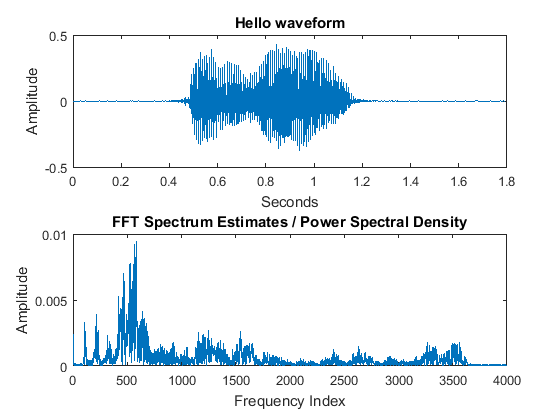
\includegraphics[width=0.75\textwidth]		
	{speech_processing/03_FFTpluswaveform}
	\caption{Waveform and FFT computed for the word "Hello".}
	\label{fig:cyka}
\end{figure}

\subsubsection{Spectrogram}
The spectrogram of the signal was computed from the FFT and it shows a visual representation of the spectrum of frequencies marked by the intensity of the color.
After the spectrogram is sliced into 25 ms chunks, it is feed as the input to the network. 
A neural network can find patterns in this data more easily than raw sound waves because certain patterns can be distinguished in the graph. Such a spectrogram can be seen in Appendix \ref{ch:appClabel}, figure \ref{fig:Spectrogram}.

\section{Modern analysis}
In the last decade, the state-of-the-art speech recognition models were phonetic-based
 approaches. Acoustic models with generative probabilistic models for sequential 
data like the Hidden Markov Model (HMM) require both text and speech data and,
furthermore a word to phoneme dictionary.
 Even though these models can be made more accurate when speech data is correlated with phoneme transcriptions, this is a gargantuan task to be attempted by hand. This makes 
 phoneme-level transcriptions less likely to be used on large data sets.
  Both  speech recognizers of the past and today  rely on segmenting sound waves, but word based processing is far more efficient in modern speech recognizer (SR) systems.
  
\subsubsection{Mel Frequency Cepstrum Coefficients}
Mel-frequency cepstral coefficients (MFCCs) are coefficients that collectively make up a Mel-frequency cepstral (MFC). 
They are taken from a cepstral representation of the audio clip by finding the spectrum of the spectrum of the original audio file.
 Compared to normal cepstrum, in MFC, the frequency bands are spaced at equal distances on the mel scale.
 This mimics a humans response to sound better that a linearly represented frequency band \cite{sahidullah2012design}.\\\\
Speech is a continuous action, where the present utterance will affect the future one. Combined with the fact that the English language is not a phonetic means that a direct
representation of each character to their sound is impossible. To overcome this problem, the neural network is trained on overlapping windows both before and after the current speech sample.\\\\
In the model developed by us, nine slices of audio are used before and after the current index, adding up to $19$ time points for each window. With $26$ cepstral coefficients, this gives $494$ data points per $25ms$ observation.
For our RNN example, we use 9 time slices before and 9 after, for a total of 19 time points per window. With 26 cepstral coefficients, this is 494 data points per 25 ms observation. Depending on the data sampling rate, $26$ cepstral features are used for $16 000 Hz$, seen in \ref{lst:MFCC}.

\begin{lstlisting}[language = Python, label=lst:MFCC, caption = Example code to obtain MFCC features.]
# Load wav files
fs, audio = wav.read(audio_filename)
 
# Get mfcc coefficients
orig_inputs = mfcc(audio, samplerate=fs, numcep=numcep)
 
# For each time slice of the training set, we need to copy the context this makes
train_inputs = np.array([], np.float32)
train_inputs.resize((orig_inputs.shape[0], numcep + 2 * numcep * numcontext))
 
for time_slice in range(train_inputs.shape[0]):
    # Pick up to numcontext time slices in the past,
    # And complete with empty mfcc features
    need_empty_past = max(0, ((time_slices[0] + numcontext) - time_slice))
    empty_source_past = list(empty_mfcc for empty_slots in range(need_empty_past))
    data_source_past = orig_inputs[max(0, time_slice - numcontext):time_slice]
    assert(len(empty_source_past) + len(data_source_past) == numcontext)
\end{lstlisting}
 
\subsection{Connectionist Temporal Classification loss function}
 Discarding the use of phonemes for neural networks can be done by switching to an
 objective function that computes predictions at the character-level transcriptions.\\\\
Connectionist Temporal Classification (CTC) provides probabilities for multiple sets, encapsulating all possible character-level transcriptions of the speech sample.
The network uses the objective function to choose the highest probability for a transcription and calculates the error rate. The error is generated by comparing the
predicted result to the absolute value of the transcript before updating the weights of the network during training \cite{Great}.\\\\
The character-level error used by the CTC loss function is different from the Levenshtein \cite{stratonovich1960conditional} word error distance that is used in traditional models. Considering that the scope of this project is limited to the English language, it is important to know
that the character versus error rate will be quite different, because English is a
non-phonetic language.